
%% bare_conf_compsoc.tex
%% V1.4b
%% 2015/08/26
%% by Michael Shell
%% See:
%% http://www.michaelshell.org/
%% for current contact information.
%%
%% This is a skeleton file demonstrating the use of IEEEtran.cls
%% (requires IEEEtran.cls version 1.8b or later) with an IEEE Computer
%% Society conference paper.
%%
%% Support sites:
%% http://www.michaelshell.org/tex/ieeetran/
%% http://www.ctan.org/pkg/ieeetran
%% and
%% http://www.ieee.org/

%%*************************************************************************
%% Legal Notice:
%% This code is offered as-is without any warranty either expressed or
%% implied; without even the implied warranty of MERCHANTABILITY or
%% FITNESS FOR A PARTICULAR PURPOSE! 
%% User assumes all risk.
%% In no event shall the IEEE or any contributor to this code be liable for
%% any damages or losses, including, but not limited to, incidental,
%% consequential, or any other damages, resulting from the use or misuse
%% of any information contained here.
%%
%% All comments are the opinions of their respective authors and are not
%% necessarily endorsed by the IEEE.
%%
%% This work is distributed under the LaTeX Project Public License (LPPL)
%% ( http://www.latex-project.org/ ) version 1.3, and may be freely used,
%% distributed and modified. A copy of the LPPL, version 1.3, is included
%% in the base LaTeX documentation of all distributions of LaTeX released
%% 2003/12/01 or later.
%% Retain all contribution notices and credits.
%% ** Modified files should be clearly indicated as such, including  **
%% ** renaming them and changing author support contact information. **
%%*************************************************************************


% *** Authors should verify (and, if needed, correct) their LaTeX system  ***
% *** with the testflow diagnostic prior to trusting their LaTeX platform ***
% *** with production work. The IEEE's font choices and paper sizes can   ***
% *** trigger bugs that do not appear when using other class files.       ***                          ***
% The testflow support page is at:
% http://www.michaelshell.org/tex/testflow/



\documentclass[conference,compsoc]{IEEEtran}
% Some/most Computer Society conferences require the compsoc mode option,
% but others may want the standard conference format.
%
% If IEEEtran.cls has not been installed into the LaTeX system files,
% manually specify the path to it like:
% \documentclass[conference,compsoc]{../sty/IEEEtran}





% Some very useful LaTeX packages include:
% (uncomment the ones you want to load)


% *** MISC UTILITY PACKAGES ***
%
%\usepackage{ifpdf}
% Heiko Oberdiek's ifpdf.sty is very useful if you need conditional
% compilation based on whether the output is pdf or dvi.
% usage:
% \ifpdf
%   % pdf code
% \else
%   % dvi code
% \fi
% The latest version of ifpdf.sty can be obtained from:
% http://www.ctan.org/pkg/ifpdf
% Also, note that IEEEtran.cls V1.7 and later provides a builtin
% \ifCLASSINFOpdf conditional that works the same way.
% When switching from latex to pdflatex and vice-versa, the compiler may
% have to be run twice to clear warning/error messages.






% *** CITATION PACKAGES ***
%
\ifCLASSOPTIONcompsoc
  % IEEE Computer Society needs nocompress option
  % requires cite.sty v4.0 or later (November 2003)
  \usepackage[nocompress]{cite}
\else
  % normal IEEE
  \usepackage{cite}
\fi
% cite.sty was written by Donald Arseneau
% V1.6 and later of IEEEtran pre-defines the format of the cite.sty package
% \cite{} output to follow that of the IEEE. Loading the cite package will
% result in citation numbers being automatically sorted and properly
% "compressed/ranged". e.g., [1], [9], [2], [7], [5], [6] without using
% cite.sty will become [1], [2], [5]--[7], [9] using cite.sty. cite.sty's
% \cite will automatically add leading space, if needed. Use cite.sty's
% noadjust option (cite.sty V3.8 and later) if you want to turn this off
% such as if a citation ever needs to be enclosed in parenthesis.
% cite.sty is already installed on most LaTeX systems. Be sure and use
% version 5.0 (2009-03-20) and later if using hyperref.sty.
% The latest version can be obtained at:
% http://www.ctan.org/pkg/cite
% The documentation is contained in the cite.sty file itself.
%
% Note that some packages require special options to format as the Computer
% Society requires. In particular, Computer Society  papers do not use
% compressed citation ranges as is done in typical IEEE papers
% (e.g., [1]-[4]). Instead, they list every citation separately in order
% (e.g., [1], [2], [3], [4]). To get the latter we need to load the cite
% package with the nocompress option which is supported by cite.sty v4.0
% and later.





% *** GRAPHICS RELATED PACKAGES ***
%
\ifCLASSINFOpdf
   \usepackage[pdftex]{graphicx}
  % declare the path(s) where your graphic files are
  % \graphicspath{{../pdf/}{../jpeg/}}
  % and their extensions so you won't have to specify these with
  % every instance of \includegraphics
  % \DeclareGraphicsExtensions{.pdf,.jpeg,.png}
\else
  % or other class option (dvipsone, dvipdf, if not using dvips). graphicx
  % will default to the driver specified in the system graphics.cfg if no
  % driver is specified.
  % \usepackage[dvips]{graphicx}
  % declare the path(s) where your graphic files are
  % \graphicspath{{../eps/}}
  % and their extensions so you won't have to specify these with
  % every instance of \includegraphics
  % \DeclareGraphicsExtensions{.eps}
\fi
% graphicx was written by David Carlisle and Sebastian Rahtz. It is
% required if you want graphics, photos, etc. graphicx.sty is already
% installed on most LaTeX systems. The latest version and documentation
% can be obtained at: 
% http://www.ctan.org/pkg/graphicx
% Another good source of documentation is "Using Imported Graphics in
% LaTeX2e" by Keith Reckdahl which can be found at:
% http://www.ctan.org/pkg/epslatex
%
% latex, and pdflatex in dvi mode, support graphics in encapsulated
% postscript (.eps) format. pdflatex in pdf mode supports graphics
% in .pdf, .jpeg, .png and .mps (metapost) formats. Users should ensure
% that all non-photo figures use a vector format (.eps, .pdf, .mps) and
% not a bitmapped formats (.jpeg, .png). The IEEE frowns on bitmapped formats
% which can result in "jaggedy"/blurry rendering of lines and letters as
% well as large increases in file sizes.
%
% You can find documentation about the pdfTeX application at:
% http://www.tug.org/applications/pdftex





% *** MATH PACKAGES ***
%
%\usepackage{amsmath}
% A popular package from the American Mathematical Society that provides
% many useful and powerful commands for dealing with mathematics.
%
% Note that the amsmath package sets \interdisplaylinepenalty to 10000
% thus preventing page breaks from occurring within multiline equations. Use:
%\interdisplaylinepenalty=2500
% after loading amsmath to restore such page breaks as IEEEtran.cls normally
% does. amsmath.sty is already installed on most LaTeX systems. The latest
% version and documentation can be obtained at:
% http://www.ctan.org/pkg/amsmath





% *** SPECIALIZED LIST PACKAGES ***
%
%\usepackage{algorithmic}
% algorithmic.sty was written by Peter Williams and Rogerio Brito.
% This package provides an algorithmic environment fo describing algorithms.
% You can use the algorithmic environment in-text or within a figure
% environment to provide for a floating algorithm. Do NOT use the algorithm
% floating environment provided by algorithm.sty (by the same authors) or
% algorithm2e.sty (by Christophe Fiorio) as the IEEE does not use dedicated
% algorithm float types and packages that provide these will not provide
% correct IEEE style captions. The latest version and documentation of
% algorithmic.sty can be obtained at:
% http://www.ctan.org/pkg/algorithms
% Also of interest may be the (relatively newer and more customizable)
% algorithmicx.sty package by Szasz Janos:
% http://www.ctan.org/pkg/algorithmicx




% *** ALIGNMENT PACKAGES ***
%
%\usepackage{array}
% Frank Mittelbach's and David Carlisle's array.sty patches and improves
% the standard LaTeX2e array and tabular environments to provide better
% appearance and additional user controls. As the default LaTeX2e table
% generation code is lacking to the point of almost being broken with
% respect to the quality of the end results, all users are strongly
% advised to use an enhanced (at the very least that provided by array.sty)
% set of table tools. array.sty is already installed on most systems. The
% latest version and documentation can be obtained at:
% http://www.ctan.org/pkg/array


% IEEEtran contains the IEEEeqnarray family of commands that can be used to
% generate multiline equations as well as matrices, tables, etc., of high
% quality.




% *** SUBFIGURE PACKAGES ***
%\ifCLASSOPTIONcompsoc
%  \usepackage[caption=false,font=footnotesize,labelfont=sf,textfont=sf]{subfig}
%\else
%  \usepackage[caption=false,font=footnotesize]{subfig}
%\fi
% subfig.sty, written by Steven Douglas Cochran, is the modern replacement
% for subfigure.sty, the latter of which is no longer maintained and is
% incompatible with some LaTeX packages including fixltx2e. However,
% subfig.sty requires and automatically loads Axel Sommerfeldt's caption.sty
% which will override IEEEtran.cls' handling of captions and this will result
% in non-IEEE style figure/table captions. To prevent this problem, be sure
% and invoke subfig.sty's "caption=false" package option (available since
% subfig.sty version 1.3, 2005/06/28) as this is will preserve IEEEtran.cls
% handling of captions.
% Note that the Computer Society format requires a sans serif font rather
% than the serif font used in traditional IEEE formatting and thus the need
% to invoke different subfig.sty package options depending on whether
% compsoc mode has been enabled.
%
% The latest version and documentation of subfig.sty can be obtained at:
% http://www.ctan.org/pkg/subfig




% *** FLOAT PACKAGES ***
%
%\usepackage{fixltx2e}
% fixltx2e, the successor to the earlier fix2col.sty, was written by
% Frank Mittelbach and David Carlisle. This package corrects a few problems
% in the LaTeX2e kernel, the most notable of which is that in current
% LaTeX2e releases, the ordering of single and double column floats is not
% guaranteed to be preserved. Thus, an unpatched LaTeX2e can allow a
% single column figure to be placed prior to an earlier double column
% figure.
% Be aware that LaTeX2e kernels dated 2015 and later have fixltx2e.sty's
% corrections already built into the system in which case a warning will
% be issued if an attempt is made to load fixltx2e.sty as it is no longer
% needed.
% The latest version and documentation can be found at:
% http://www.ctan.org/pkg/fixltx2e


%\usepackage{stfloats}
% stfloats.sty was written by Sigitas Tolusis. This package gives LaTeX2e
% the ability to do double column floats at the bottom of the page as well
% as the top. (e.g., "\begin{figure*}[!b]" is not normally possible in
% LaTeX2e). It also provides a command:
%\fnbelowfloat
% to enable the placement of footnotes below bottom floats (the standard
% LaTeX2e kernel puts them above bottom floats). This is an invasive package
% which rewrites many portions of the LaTeX2e float routines. It may not work
% with other packages that modify the LaTeX2e float routines. The latest
% version and documentation can be obtained at:
% http://www.ctan.org/pkg/stfloats
% Do not use the stfloats baselinefloat ability as the IEEE does not allow
% \baselineskip to stretch. Authors submitting work to the IEEE should note
% that the IEEE rarely uses double column equations and that authors should try
% to avoid such use. Do not be tempted to use the cuted.sty or midfloat.sty
% packages (also by Sigitas Tolusis) as the IEEE does not format its papers in
% such ways.
% Do not attempt to use stfloats with fixltx2e as they are incompatible.
% Instead, use Morten Hogholm'a dblfloatfix which combines the features
% of both fixltx2e and stfloats:
%
% \usepackage{dblfloatfix}
% The latest version can be found at:
% http://www.ctan.org/pkg/dblfloatfix




% *** PDF, URL AND HYPERLINK PACKAGES ***
%
%\usepackage{url}
% url.sty was written by Donald Arseneau. It provides better support for
% handling and breaking URLs. url.sty is already installed on most LaTeX
% systems. The latest version and documentation can be obtained at:
% http://www.ctan.org/pkg/url
% Basically, \url{my_url_here}.




% *** Do not adjust lengths that control margins, column widths, etc. ***
% *** Do not use packages that alter fonts (such as pslatex).         ***
% There should be no need to do such things with IEEEtran.cls V1.6 and later.
% (Unless specifically asked to do so by the journal or conference you plan
% to submit to, of course. )


% correct bad hyphenation here
\hyphenation{op-tical net-works semi-conduc-tor}
\usepackage{float}

\begin{document}
%
% paper title
% Titles are generally capitalized except for words such as a, an, and, as,
% at, but, by, for, in, nor, of, on, or, the, to and up, which are usually
% not capitalized unless they are the first or last word of the title.
% Linebreaks \\ can be used within to get better formatting as desired.
% Do not put math or special symbols in the title.
\title{A Study on Different Machine Learning Models To Predict Breast Cancer}


% author names and affiliations
% use a multiple column layout for up to three different
% affiliations
%\author{\IEEEauthorblockN{N. Safiyyah}
%\IEEEauthorblockA{School of Computing Science \\and Engineering\\
%VIT Chennai\\
%TamilNadu\\India 600127\\

%\and
%\IEEEauthorblockN{A. Shahina}
%\IEEEauthorblockA{SSN College of Engineering\\
%Kalavakkam, Chennai\\
%TamilNadu\\India 600127
%Email: homer@thesimpsons.com}
%\and
%\IEEEauthorblockN{James Kirk\\ and Montgomery Scott}
%\IEEEauthorblockA{Starfleet Academy\\
%San Francisco, California 96678-2391\\
%Telephone: (800) 555--1212\\
%Fax: (888) 555--1212}}

% conference papers do not typically use \thanks and this command
% is locked out in conference mode. If really needed, such as for
% the acknowledgment of grants, issue a \IEEEoverridecommandlockouts
% after \documentclass

% for over three affiliations, or if they all won't fit within the width
% of the page (and note that there is less available width in this regard for
% compsoc conferences compared to traditional conferences), use this
% alternative format:
% 
\author{\IEEEauthorblockN{Shashank Pathak(15BCE1287)\IEEEauthorrefmark{1},
%Eldon Tyrell\IEEEauthorrefmark{4}}
\IEEEauthorblockA{\IEEEauthorrefmark{1}School of Computing Sciences and Engineering, 
%	\IEEEauthorrefmark{4} School of Advanced Sciences\\
VIT Chennai, Tamilnadu, India 600127\\
Email: shashank.pathak2015@vit.ac.in\IEEEauthorrefmark{1}}
}
%Atlanta, Georgia 30332--0250\\ Email: see http://www.michaelshell.org/contact.html}
%\IEEEauthorblockA{\IEEEauthorrefmark{3}Starfleet Academy, San Francisco, California 96678-2391\\
%Telephone: (800) 555--1212, Fax: (888) 555--1212}
%\IEEEauthorblockA{\IEEEauthorrefmark{4}Tyrell Inc., 123 Replicant Street, Los Angeles, California 90210--4321}}

}


% use for special paper notices
%\IEEEspecialpapernotice{(Invited Paper)}




% make the title area
\maketitle
\\


% As a general rule, do not put math, special symbols or citations
% in the abstract
\begin{abstract}
	Breast Cancer is one of the most widespread disease
among woman worldwide. Early and Accurate diagnosis of breast cancer is an extremely important step in rehabilitation and
treatment. However, it is not an easy task due to several 
factors that play a big role  in detection of a cancerous tumour. Machine learning techniques are prominently used in disease detection phases as it gives quite accurate results. Various
techniques may provide different desired accuracies and
it is therefore imperative to use the most suitable method
which provides the best desired results. This research paper
seeks to provide comparative analysis of Artificial Neural Network,Support Vector Machine,Decision Tree(ID3),K Means,K nearest Neigbours,Logistic Regression and Perceptron on the Wisconsin breast cancer dataset
\\
\end{abstract}

% no keywords




% For peer review papers, you can put extra information on the cover
% page as needed:
% \ifCLASSOPTIONpeerreview
% \begin{center} \bfseries EDICS Category: 3-BBND \end{center}
% \fi
%
% For peerreview papers, this IEEEtran command inserts a page break and
% creates the second title. It will be ignored for other modes.
%\IEEEpeerreviewmaketitle



\section{Introduction}
% no \IEEEPARstart

% You must have at least 2 lines in the paragraph with the drop letter
% (should never be an issue)

According to different survey and WHO 25\% of the females in the US are diagnosed with breast cancer at some stage in their life. Predicting a cancerous tumor remains a challenging task for many doctors.Thus the early detection of cancerous tumour is  very important as it eases the removal of tumour and chances of survival increases.There are many factors which play  an important role in the detection of cancer but the accurate detection is not dependent on any one factor or there is no matematical formula or ratio that predicts the Breast cancer.Therefore a learning approach is required to tackle this problem.    
Machine Learning (ML), is a subfield of Artificial Intelligence (AI) that allows machines to learn without explicit
programming by exposing them to sets of data allowing
them to learn a specific task through experience.Nowadays Machine Learning is used every where from social networks to self driving car.So we will use different machine learning models like Artificial Neural Network,Support Vector Machine,Decision Tree(ID3),K Means,K nearest Neigbours,Logistic Regression and Perceptron inorder to predict that a tumour is cancerous or non-cancerous that corresponds to Malignant or Benign tumour respectively.



\section{Methodology}
	We took the Breast cancer Wisconsin dataset and realized that this dataset needed cleaning.So we cleaned the dataset by removing NaN and '?' enteries .We then analysed the dataset and calculated various stastical measures for analysing the data distribution like mean,mode,median,total valid instances etc.After this we played with the data to get some insight on data and any kind relation between class and attributes .After this we applied different Machine Learning Models like Artificial Neural Network,Support Vector Machine,Decision Tree(ID3),K Means,K nearest Neigbours,Logistic Regression and Perceptron on the dataset.We got the insample and test sample accuracies for all the models  which helped us to comparatively analyze the models for the Breast Cancer predication problem.
 

\section{Database - Breast Cancer Wisconsin Dataset(Original)}
The  Wisconsin  Breast  Cancer  datasets  from  the  UCI Machine  Learning  Repository  is  used,to  distinguish malignant (cancerous) from benign (non-cancerous) samples.This dataset consist of 699 instances and 11 attributes that would help the classiy the data into the two classes.458 of the cases are
benign and 241 are malignant.The attributes are described in the fig.1

\begin{figure}[H]
\centering
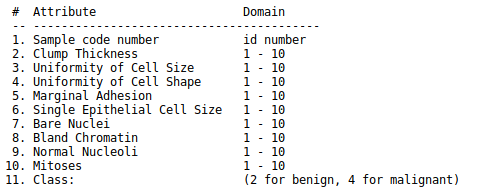
\includegraphics[width=3.5in,height=1.8in]{1.png}
% where an .eps filename suffix will be assumed under latex, 
% and a .pdf suffix will be assumed for pdflatex; or what has been declared
% via \DeclareGraphicsExtensions.
\caption{Breast Cancer Wisconsin Dataset Attributes}
\label{fig_error}

\end{figure}  
 The above attributes except for the class are of integer type, and their values range between 1 and 10 both inclusive. The class attribute has a value of 2 for benign and 4 for malignant.  

\section{Classification Algorithms}
The various algorithms used in this study are explained briefly in this section of the document
\newline

i)Decision Tree
\newline
\par
Decision tree is used in supervised learning in machine learning for classification.Decision tree is like a normal tree that is used in data structures whose nodes  represent as features or attributes,branches are the various conditions on which classification is done,leaves represent the classes of the dataset.So decision tree starts from start node which are non terminal goes through the branches which are the various classification conditions and reaches the leaves which are the classes of the data.Each node contains a condition which decide which branch to follow next.
\par
The nodes are created using the entropy or information gain values.The condition on the nodes decide the path if the condition is satisfied then that path is followed otherwise different path is taken by the algorithm.
Algorithm starts from the root node and follows a top down approach to traverse through the tree to reach the nodes.
\par 
We have used ID3 Algorithm to create the decision tree for classification.In ID3 algorithm it searches for that attribute which classify the most number of data instances that is it chooses that attribute which is able to classify most efficiently and then it makes tree subsequently in order in which these attributes classify the data using entropy and information gain of each attribute.The algorithm continues the process until finding subset instances belonging to the same class, and so the leaf node is created, and the algorithm stops when it has handled all the attributes.

\newline

ii)K Nearest Neighbor
\newline
\par
\begin{figure}[H]
\centering

\includegraphics[width=3.5in,height=0.4in]{knn1.png}
% where an .eps filename suffix will be assumed under latex, 
% and a .pdf suffix will be assumed for pdflatex; or what has been declared
% via \DeclareGraphicsExtensions.
\caption{Euclidean Distance used in KNN}
\label{fig_error}

\end{figure}  
(KNN) K Nearest Neighbor classifier is one of the basic classifiers in  machine learning algorithms.It classifies the data based on the majority vote of the K nearest points of a data point.Basically what it does is that it maps all the data instances in the n dimension space and calculates the distance between a given point and other points  k and find out the K nearest neighbours  and then it takes votes of the classes of these neighbours and if there are more number of points which are belonging to a particular class t then the class of the point is t.
It is a supervised learning mechanism so we need to decide the value of K which is used by the algorithm for classification.
\newline


iii)Support Vector Machines
\begin{figure}[H]
\centering
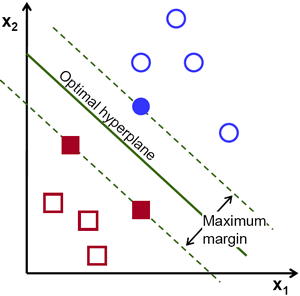
\includegraphics[width=3in,height=1.8in]{svm1.png}
% where an .eps filename suffix will be assumed under latex, 
% and a .pdf suffix will be assumed for pdflatex; or what has been declared
% via \DeclareGraphicsExtensions.
\caption{Support Vector Machine}
\label{fig_error}

\end{figure}  
\newline
\par
SVM(Support Vector Machines) is a very important and efficient suprevised learning algorithm in machine learning.Support Vectors are the critical sample points which are used to generate a linear function which divides the points as broadly as possible.These support vectors are used for deciding the width of the boundary of the linear function.The more will be the boundary of this linear function the more better will be the classification.So we aim for maximizing the boundary and this is also known as maximum margin classifier.SVM aims to find the most suitable hyperplane that divided the dataset into different classes.
\newline
\begin{figure}[H]
\centering
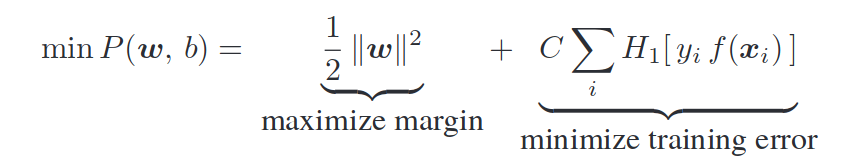
\includegraphics[width=3.5in,height=0.6in]{svm2.png}
% where an .eps filename suffix will be assumed under latex, 
% and a .pdf suffix will be assumed for pdflatex; or what has been declared
% via \DeclareGraphicsExtensions.
\caption{SVM Maximize the margin}
\label{fig_error}

\end{figure}  

iv)Multi Layer Perceptron
\begin{figure}[H]
\centering
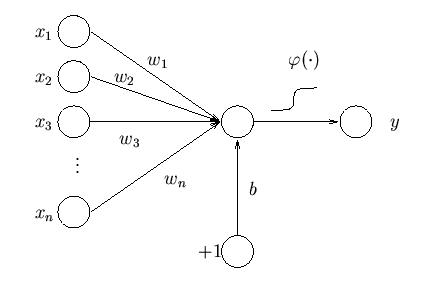
\includegraphics[width=3.5in,height=1.8in]{mlp1.png}
% where an .eps filename suffix will be assumed under latex, 
% and a .pdf suffix will be assumed for pdflatex; or what has been declared
% via \DeclareGraphicsExtensions.
\caption{Multi Layered Perceptron}
\label{fig_error}

\end{figure}  
\newline
\par
MLP(Multi Layer Perceptron) is a supervised classification algorithm used in machine learning.Multi Layer perceptron  is a feedforward neural network with one or more layers between input and output layer.The algorithm uses a feedforward approach in which data starts from the input layer and flows till it reaches the output layer. This type of network is trained with the backpropagation learning algorithm.Once a feedforward cycle is complete we calculate the error between the predicted value and the value of the class at the output layer and then this error is propagated backward till it reaches the last layer and the weights of the neural nets are modified according to the error.
\par
\begin{figure}[H]
\centering
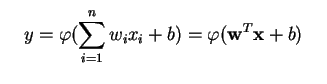
\includegraphics[width=3.5in,height=0.6in]{mlp2.png}
% where an .eps filename suffix will be assumed under latex, 
% and a .pdf suffix will be assumed for pdflatex; or what has been declared
% via \DeclareGraphicsExtensions.
\caption{Forward propogation in MLP}
\label{fig_error}

\end{figure}  
So the algorithm perform in cycles where one complete cycle consist of feedforward the network calculating the error and backpropagation of error and the updation of weights of neurons.These are the basic three steps which complete a given cycle.Linearly inseperable problems can be solved using Multi Layer Perceptron.MLP uses stochastic gradient descent for classification.
\newline


v)K Means

\newline
K means algorithm is  distance based classification.There are two main step in K means classification first step is cluster assignment step and the second step is updation of centroid.We need to define K for the algorithm.In K means algorithm distance of the given data point is taken with all the other data points and the centroid of the group is decided using the data points that belong to the same class and then we update the centroid with each step.K means is an iterative algorithm.



\newline
vi)Logistic Regression

\newline
Logistic Regression is a supervised machine learning algorithm which gives a probabilistic approach to machine learning.Logistic regression values range between zero and one.Logistic Regression gives the probability of a point belonging to a particular class.We estimate teh value of the coefficients using the stochastic gradient descent.
We can estimate the values of the coefcients using stochastic gradient descent. This is a simple procedure that can be used by many algorithms in machine learning. It works by using the model to calculate a prediction for each instance in the training set and calculating the error for each prediction. We can apply stochastic gradient descent to the problem of finding the coefcients for the logistic regression model as follows by calculating for each instance a prediction using the current value of coefficents and calculating new coefficeints based on the error in the prediction.The process is repeated until the model is accurate enough or for a fixed number of iterations.
\begin{figure}[H]
\centering
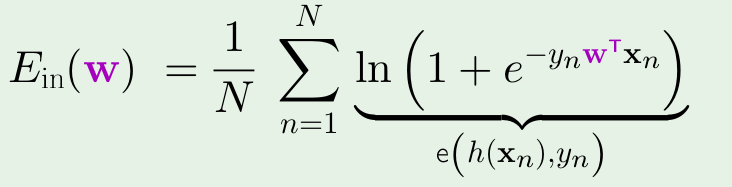
\includegraphics[width=3.5in,height=0.6in]{lr1.png}
% where an .eps filename suffix will be assumed under latex, 
% and a .pdf suffix will be assumed for pdflatex; or what has been declared
% via \DeclareGraphicsExtensions.
\caption{Logistic Regression}
\label{fig_error}

\end{figure}  

\newline
vii)Perceptron
\newline
\par
Perceptron is the most basic algorithm under supervised classification. It involves the mapping of a function on its input x (a real- valued vector) to an output f(x) (a single binary value):
where w is the vector of a real-valued weights and b is the bias.
The bias shifts the decision boundary away from the origin and does not depend on any input value.

This linear function is used to classify the in-sample as well as out-sample data and the score of this algorithm can be calculated using the number of misclassification done by the best hypothesis.




\section{Experiments}
We took the Breast cancer Wisconsin dataset and realized that this dataset needed cleaning.So we cleaned the dataset by removing NaN and '?' enteries.After this we used standard scaler to scale the values although this step is not necessary as the range of attributes are already between 1 to 10. After this we changed the label value of benign and Malignant from 2 and 4 to -1 and 1 repectively as this is a case of binary classification and it would be better to have a positive and a negative case.Then we used train\_test\_split from cross\_validation of scikit learn to split the dataset into X\_train,y\_train X\_test and y\_test.
From plotting and infographics we used seaborn and matplotlib for all the models.
\par
 After this we made a perceptron from scratch for our dataset and trained it on the X\_train and y\_train.We got a seprating hyperplane as in fig. .After this we analysed the performance of perceptron for differnt value of epochs.
 \begin{figure}[H]
\centering
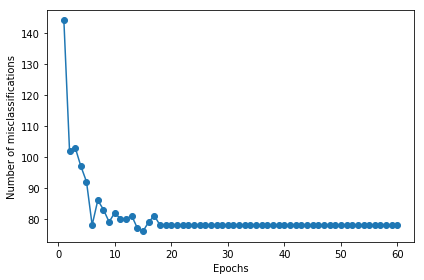
\includegraphics[width=3.5in,height=1.8in]{p2.png}
% where an .eps filename suffix will be assumed under latex, 
% and a .pdf suffix will be assumed for pdflatex; or what has been declared
% via \DeclareGraphicsExtensions.
\caption{Misclassification vs errors}
\label{fig_error}

\end{figure}
\begin{figure}[H]
\centering
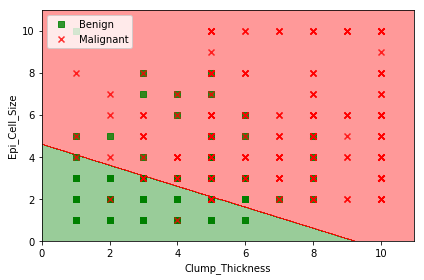
\includegraphics[width=3.5in,height=1.8in]{p3.png}
% where an .eps filename suffix will be assumed under latex, 
% and a .pdf suffix will be assumed for pdflatex; or what has been declared
% via \DeclareGraphicsExtensions.
\caption{Classification by Perceptron}
\label{fig_error}

\end{figure}    
\par
After this we trained Decision tree on our training dataset for all attributes.After doing some hyperparameter tuning we concluded the optimum value of max\_depth equal to 4.After this we used the testing dataset to test the ID3 based Decision tree and got a accuracy of 95.9\%.
\begin{figure}[H]
\centering
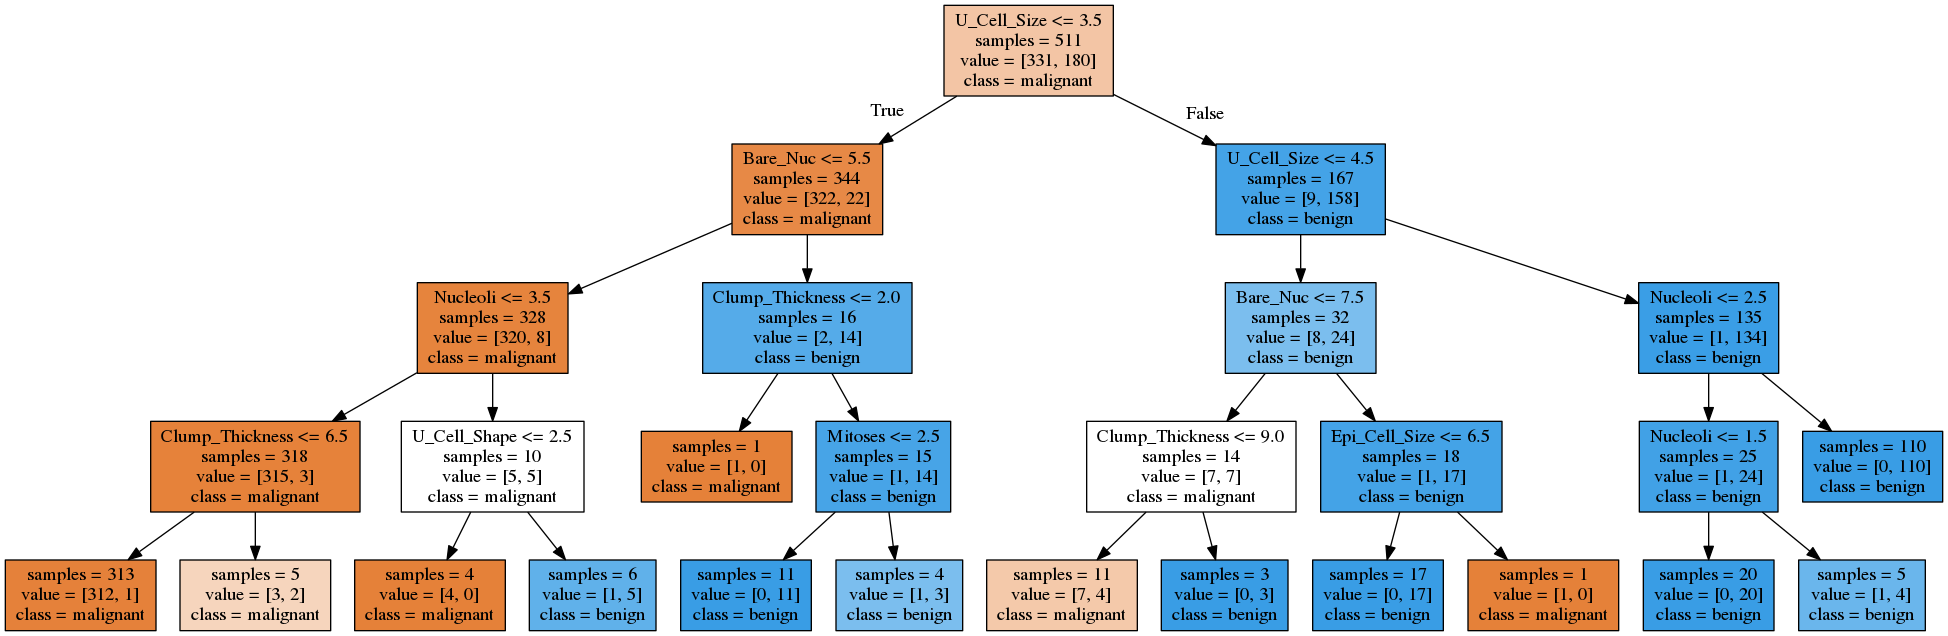
\includegraphics[width=3.5in,height=1.8in]{DecisionTree.png}
% where an .eps filename suffix will be assumed under latex, 
% and a .pdf suffix will be assumed for pdflatex; or what has been declared
% via \DeclareGraphicsExtensions.
\caption{Classification by Decision Tree}
\label{fig_error}

\end{figure}  
\par
Then we applied Logistic Regression model from sklearn models and trained it on  X\_train and y\_train. After this we used the score method to test the trained Logistic Regressor and got around 32\% accuracy which is the lowest of all the model we used.
\begin{figure}[H]
\centering
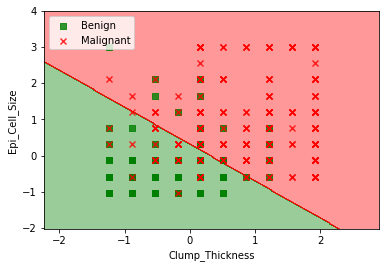
\includegraphics[width=3.5in,height=1.8in]{lr2.png}
% where an .eps filename suffix will be assumed under latex, 
% and a .pdf suffix will be assumed for pdflatex; or what has been declared
% via \DeclareGraphicsExtensions.
\caption{Classification by Logistic Regression}
\label{fig_error}

\end{figure}  
\par
After this we tried an unsupervised learning model i.e. K Means to
find the clusters in our dataset and got 2 clusters and a distotion of aroun 347.49.The hyper parameter values  are mentioned in the table.
\begin{figure}[H]
\centering
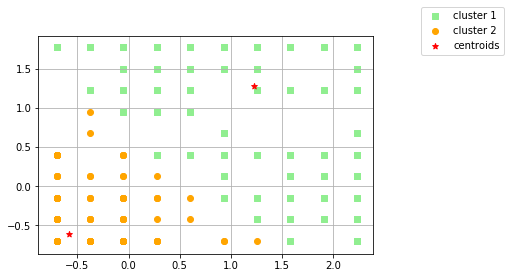
\includegraphics[width=3.5in,height=1.8in]{km2.png}
% where an .eps filename suffix will be assumed under latex, 
% and a .pdf suffix will be assumed for pdflatex; or what has been declared
% via \DeclareGraphicsExtensions.
\caption{Clustering by K Means}
\label{fig_error}

\end{figure}  
\begin{figure}[H]
\centering
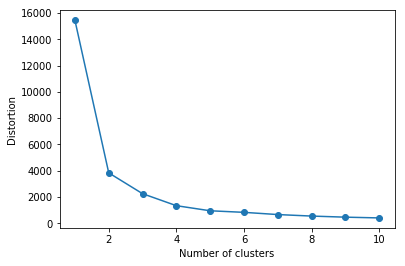
\includegraphics[width=3.5in,height=1.8in]{km3.png}
% where an .eps filename suffix will be assumed under latex, 
% and a .pdf suffix will be assumed for pdflatex; or what has been declared
% via \DeclareGraphicsExtensions.
\caption{no.of clusters vs Distortion}
\label{fig_error}

\end{figure}  
\par
After we used multi layered perceptron or more commonly known as Artificial neural network.We trained our model for 1000 epochs and 25 hidden layers to get a 2 neuron output layer.Then we tested the model on  X\_test and y\_test and got 97.56\% accuracy.
\begin{figure}[H]
\centering
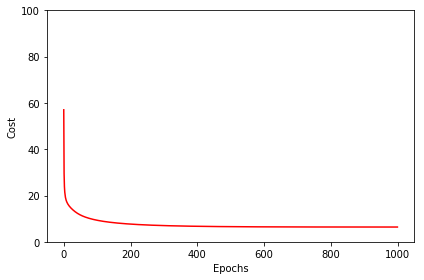
\includegraphics[width=3.5in,height=1.8in]{mlp3.png}
% where an .eps filename suffix will be assumed under latex, 
% and a .pdf suffix will be assumed for pdflatex; or what has been declared
% via \DeclareGraphicsExtensions.
\caption{Cost vs Epochs in MLP}
\label{fig_error}

\end{figure}  
\par
Then we tried support vector machine for the Breast cancer prediction problem. This is the most widely used model for this problem and we used the SVM from sklearn model library.We tried different kernels like radial bias,polynomial and linear.We used Gridsearch and pipeline to do hyper parameter tuning and check the best kernel.We got best results for rbf kernel and for C i.e. the cost of error value equal to 10.We got a accuracy of 94.63\%
\begin{figure}[H]
\centering
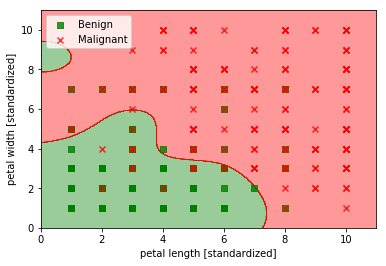
\includegraphics[width=3.5in,height=1.8in]{svm3.png}
% where an .eps filename suffix will be assumed under latex, 
% and a .pdf suffix will be assumed for pdflatex; or what has been declared
% via \DeclareGraphicsExtensions.
\caption{Classification by SVM}
\label{fig_error}

\end{figure}  
\par
The last model that we tried was K Nearest Neighbour.After training on our dataset we did the hyperparameter tuning using  cross\_val\_score of scikitlearn to get the best parameters.We got no. of neighbours equal to 2.We used Minkowski distance as the distance parameter .After testing the model on  X\_test and y\_test we got a accuracy of 96.09\%
\begin{figure}[H]
\centering
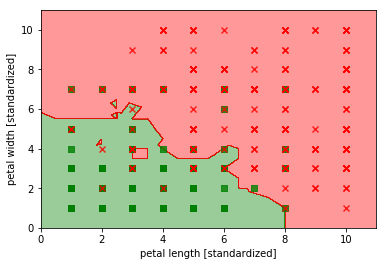
\includegraphics[width=3.5in,height=1.8in]{knn2.png}
% where an .eps filename suffix will be assumed under latex, 
% and a .pdf suffix will be assumed for pdflatex; or what has been declared
% via \DeclareGraphicsExtensions.
\caption{Classification by KNN}
\label{fig_error}

\end{figure}  
 


\section{Conclusion}

\begin{figure}[H]
\centering
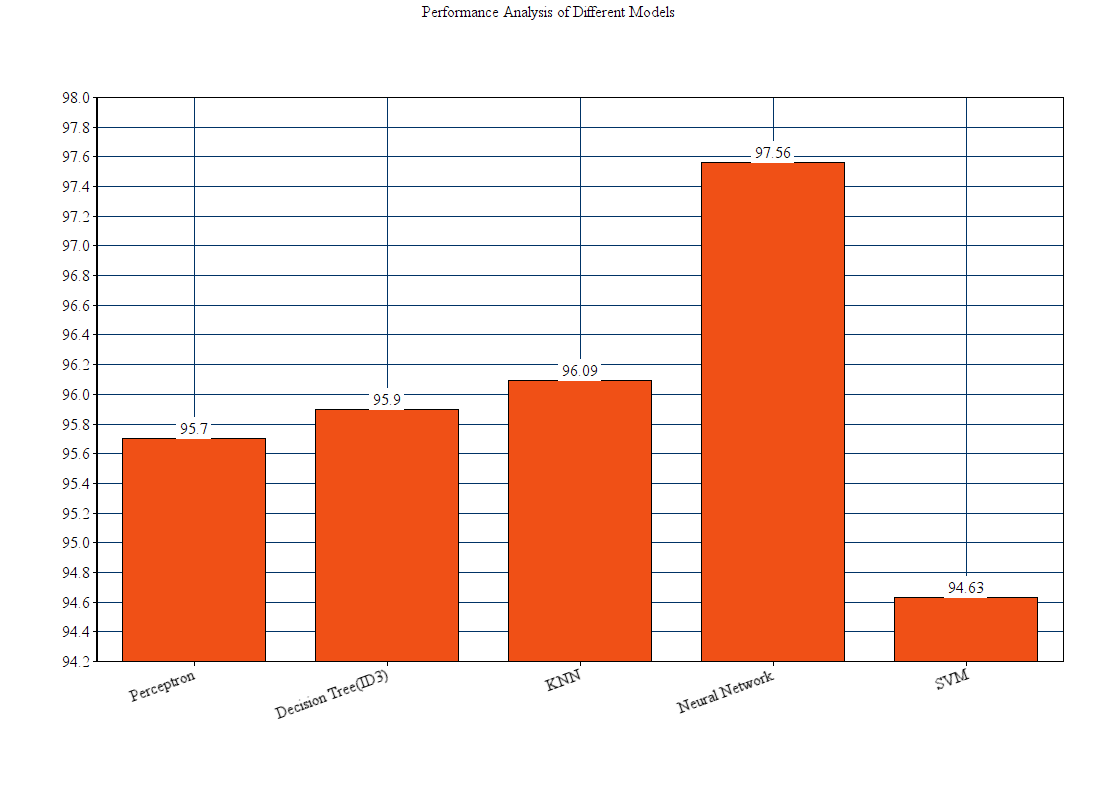
\includegraphics[width=3.5in,height=3in]{analysis_chart.png}
% where an .eps filename suffix will be assumed under latex, 
% and a .pdf suffix will be assumed for pdflatex; or what has been declared
% via \DeclareGraphicsExtensions.
\caption{Accuracies for different models}
\label{fig_error}

\end{figure}  
We trained some of the Machine Learning Models like Artificial Neural Network,Support Vector Machine,Decision Tree(ID3),K Means,K nearest Neigbours,Logistic Regression and Perceptron and got differnt accuracies.We got accuracies that are mentioned in the fig17.We can clearly see that Neural Network performed the best with accuracy 97.63\%.Most of the algorithm performed very well in the learning process but Logistic regression performed below par with wort accuracy of 32.1\%.So in this we have seen that the breast cancer dataset can be learned by most of these models very effectively.Hence the Breast Cancer Dataset is easily classifiable
using htese models. 



\section{References}
\newline
[1] WHO — Breast Cancer: Prevention and Control (2015) Retrieved
20 Jan 2015, from WHO — World Health Organization. http://
www.who.int/cancer/detection/breastcancer/en/index1.html
\newline
[2] Y. Elobaid, T.-C. Aw, J. N. W. Lim, S. Hamid, and M. Grivna, “Breast
cancer presentation delays among Arab and national women in the UAE,
a qualitative study,” SSM - Popul. Heal., Mar. 2016.
\newline
[3] E. D. Michie, D. J. Spiegelhalter, and C. C. Taylor, “Machine Learning
, Neural and Statistical Classification,” Proceeding, 1994.
\newline
[4] I. Kononenko, “Machine learning for medical diagnosis: history , state
of the art and perspective,” vol. 23, 2001.
\newline
[5] G. Williams, “Descriptive and Predictive Analytics”, Data Min. with
Ratt. R Art Excav. Data Knowl. Discov. Use R, pp. 193-203, 2011.
\newline
[6] K. Kourou, T. P. Exarchos, K. P. Exarchos, M. V. Karamouzis, and
D. I. Fotiadis, “Machine learning applications in cancer prognosis and
prediction,” Comput. Struct. Biotechnol. J., vol. 13, pp. 8-17, 2015.
\newline
[7] T. J. Cleophas and A. H. Zwinderman, “Machine Learning in Medicine,”
pp. 1-271, 2013.
\newline
[8] Y. Yasui and X. Wang, Statistical Learning from a Regression Perspec-
tive by BERK, R. A., vol. 65, no. 4. 2009.
\newline
[9]M. Lichman, UCI Machine Learning Repositry, 2013. [Online]. Available: https://archive.ics.uci.edu/.
\newline
[10] T. Fushiki, “Estimation of prediction error by using K-fold cross-
validation,” Stat. Comput., vol. 21, no. 2, pp. 137-146, 2011.
% An example of a floating figure using the graphicx package.
% Note that \label must occur AFTER (or within) \caption.
% For figures, \caption should occur after the \includegraphics.
% Note that IEEEtran v1.7 and later has special internal code that
% is designed to preserve the operation of \label within \caption
% even when the captionsoff option is in effect. However, because
% of issues like this, it may be the safest practice to put all your
% \label just after \caption rather than within \caption{}.
%
% Reminder: the "draftcls" or "draftclsnofoot", not "draft", class
% option should be used if it is desired that the figures are to be
% displayed while in draft mode.
%
%\begin{figure}[!t]
%\centering
%\includegraphics[width=2.5in]{myfigure}
% where an .eps filename suffix will be assumed under latex, 
% and a .pdf suffix will be assumed for pdflatex; or what has been declared
% via \DeclareGraphicsExtensions.
%\caption{Simulation results for the network.}
%\label{fig_sim}
%\end{figure}

% Note that the IEEE typically puts floats only at the top, even when this
% results in a large percentage of a column being occupied by floats.


% An example of a double column floating figure using two subfigures.
% (The subfig.sty package must be loaded for this to work.)
% The subfigure \label commands are set within each subfloat command,
% and the \label for the overall figure must come after \caption.
% \hfil is used as a separator to get equal spacing.
% Watch out that the combined width of all the subfigures on a 
% line do not exceed the text width or a line break will occur.
%
%\begin{figure*}[!t]
%\centering
%\subfloat[Case I]{\includegraphics[width=2.5in]{box}%
%\label{fig_first_case}}
%\hfil
%\subfloat[Case II]{\includegraphics[width=2.5in]{box}%
%\label{fig_second_case}}
%\caption{Simulation results for the network.}
%\label{fig_sim}
%\end{figure*}
%
% Note that often IEEE papers with subfigures do not employ subfigure
% captions (using the optional argument to \subfloat[]), but instead will
% reference/describe all of them (a), (b), etc., within the main caption.
% Be aware that for subfig.sty to generate the (a), (b), etc., subfigure
% labels, the optional argument to \subfloat must be present. If a
% subcaption is not desired, just leave its contents blank,
% e.g., \subfloat[].


% An example of a floating table. Note that, for IEEE style tables, the
% \caption command should come BEFORE the table and, given that table
% captions serve much like titles, are usually capitalized except for words
% such as a, an, and, as, at, but, by, for, in, nor, of, on, or, the, to
% and up, which are usually not capitalized unless they are the first or
% last word of the caption. Table text will default to \footnotesize as
% the IEEE normally uses this smaller font for tables.
% The \label must come after \caption as always.
%
%\begin{table}[!t]
%% increase table row spacing, adjust to taste
%\renewcommand{\arraystretch}{1.3}
% if using array.sty, it might be a good idea to tweak the value of
% \extrarowheight as needed to properly center the text within the cells
%\caption{An Example of a Table}
%\label{table_example}
%\centering
%% Some packages, such as MDW tools, offer better commands for making tables
%% than the plain LaTeX2e tabular which is used here.
%\begin{tabular}{|c||c|}
%\hline
%One & Two\\
%\hline
%Three & Four\\
%\hline
%\end{tabular}
%\end{table}


% Note that the IEEE does not put floats in the very first column
% - or typically anywhere on the first page for that matter. Also,
% in-text middle ("here") positioning is typically not used, but it
% is allowed and encouraged for Computer Society conferences (but
% not Computer Society journals). Most IEEE journals/conferences use
% top floats exclusively. 
% Note that, LaTeX2e, unlike IEEE journals/conferences, places
% footnotes above bottom floats. This can be corrected via the
% \fnbelowfloat command of the stfloats package.



% conference papers do not normally have an appendix



% use section* for acknowledgment
\ifCLASSOPTIONcompsoc
  % The Computer Society usually uses the plural form
%  \section*{Acknowledgments}
%\else
  % regular IEEE prefers the singular form
%  \section*{Acknowledgment}
\fi


%The authors would like to thank...





% trigger a \newpage just before the given reference
% number - used to balance the columns on the last page
% adjust value as needed - may need to be readjusted if
% the document is modified later
%\IEEEtriggeratref{8}
% The "triggered" command can be changed if desired:
%\IEEEtriggercmd{\enlargethispage{-5in}}

% references section

% can use a bibliography generated by BibTeX as a .bbl file
% BibTeX documentation can be easily obtained at:
% http://mirror.ctan.org/biblio/bibtex/contrib/doc/
% The IEEEtran BibTeX style support page is at:
% http://www.michaelshell.org/tex/ieeetran/bibtex/
%\bibliographystyle{IEEEtran}
% argument is your BibTeX string definitions and bibliography database(s)
%\bibliography{IEEEabrv,../bib/paper}
%
% <OR> manually copy in the resultant .bbl file
% set second argument of \begin to the number of references
% (used to reserve space for the reference number labels box)%
%\begin{thebibliography}{1}

%\bibitem{IEEEhowto:kopka}
%H.~Kopka and P.~W. Daly, \emph{A Guide to \LaTeX}, 3rd~ed.\hskip 1em plus
%  0.5em minus 0.4em\relax Harlow, England: Addison-Wesley, 1999.

%\bibitem{Laser:butter} Charles D. Butter, \emph{Fiber optic intruder alarm system}, Patent US 4297684 A, issued, Oct 27, 1981
%\end{thebibliography}



\bibliographystyle{IEEEtran}
\bibliography{perceptronBib}


% that's all folks
\end{document}


